%-*- coding: UTF-8 -*-
\documentclass[hpyerref,UTF8,a4paper,titlepage,12pt,oneside]{ctexbook}
\usepackage{hyperref}
\usepackage{geometry}
\usepackage{xeCJK, fontspec, xunicode, xltxtra,ulem}
\usepackage{amsthm}
\usepackage{amsmath}
\usepackage{amssymb}
\usepackage{mathrsfs}
\usepackage{mathtools}
\usepackage{commath}
\usepackage{listings}
\usepackage{float}
\usepackage{xcolor}
\usepackage{mdframed}

\graphicspath{{images/}}
\geometry{a4paper,bottom=2cm}

\title{MVSNet}
\author{陈国庆}
\date{\today}

\bibliography{plain}

% 定理结构
\theoremstyle{definition}
\newtheorem{definition}{定义}[section]
\newtheorem{theorem}{定理}[section]
\newtheorem{corollary}{推论}[theorem]
\newtheorem{lemma}[theorem]{Lemma}
\renewcommand\qedsymbol{$\blacksquare$}

\begin{document}

\maketitle
\tableofcontents

\section{齐次坐标}
	齐次坐标就是在原坐标后面添加一个维度,值为1,例如2D点$(x,y)^T$的齐次坐标为$(x,y,z)$,3D点$(x,y,z)$的齐次坐标为$(x,y,z,1)$。\\

	如果已知$(x,y,z,w)$是齐次坐标,转回3D坐标为$(x/w,y/w,z/w)$,即除以最后一维。\\

	基于这个定义齐次坐标$k(x,y,z,1)$所代表的3D坐标都是相同的。因此齐次坐标只是关注元素之间的比率,这也是“齐次”的由来。\\

	当我们拿到一个坐标$(x,y,z)$时,首先要弄明白这是个3D坐标还是2D坐标的齐次形式,这两者意义完全不同。\\

	如果已知$(x,y,0)$为齐次坐标,根据定义对应的2D坐标是$(x/0,y/0)$,这个有什么意义呢?\\

	解释这个问题,可以考虑$(x,y,\delta), \delta\rightarrow 0$对应的2D坐标,
	$$
		p = \lim_{\delta\rightarrow 0} (x/\delta, y/\delta)
	$$

	当$\delta\rightarrow 0$,$p$点会沿着$(x,y)$方向趋向于无穷,所以$(x,y,0)$为$(x,y)$方向的\textbf{无穷远点}。\\

	当拍摄照片时,可以拍到很远的场景,那些点是现实世界中的无穷远点,但他们在图像上又是真实存在像素坐标。所以相机成像可以把无穷远点映射为有限点。\\

	通过齐次坐标可以很容易表示无穷远,那么两条平行线是否交于无穷远点呢?

	\subsubsection*{线面的齐次表示}
		2D空间的直线$l$,$ax_1 + bx_2 +c =0$,方程两端乘以任意一个非0因子,都不影响直行的表示,所以$(a,b,c)^T$可表示直线$l$的齐次坐标;点$p$在直线上则表示为$p^Tl = 0$;\\

		3D空间的平面$\pi$,$ax_1 + bx_2 + cx_3 +d = 0$也可用齐次坐标$(a,b,c,d)^T$来表示,$p^T\pi = 0$也表示点$p$在面$\pi$上。\\

		如此,两条直线$l,l^\prime$的交点$q$,则可用叉乘来表示$q = l\times l^prime$。\\

		$l=(a,b,c)^T, l^\prime = (a,b,d)^T$,为两条平行直线,其交点为,
		
		\begin{equation}
			l\times l^{\prime} = 
							\begin{vmatrix}
								i & j& k \\
								a & b& c\\
								a & b& d
							\end{vmatrix}
			= (bd-bc, ac-ad, 0)^T
		\end{equation}

		的确是一个无穷远点。

	\subsubsection*{虚圆点}		
		有两个特殊的无穷远点,$(1,i,0)^T, (1,-i,0)^T$称为\textbf{虚圆点};我们考虑一下平面上圆的方程,
		$$
			(x - a)^2 + (y - b)^2 = r^2
		$$
		如果用二维齐次坐标可表示为,
		$$
			(x - aw)^2 + (y - bw)^2 = r^2w^2
		$$

		两个椭圆有4个交点,两个圆有2个交点,大家都是二次方程,为啥圆只有2个交点?缺的两个点就是虚圆点,他们在无穷远处相交。

	\subsubsection*{无穷远线面}
		经过简单验证可知,任意的无穷远点都在$l_{\infty} = (0,0,1)^T$上,称为\textbf{无穷远线};同理所有无穷远直线汇聚成无穷远面$\pi_{\infty} = (0,0,0,1)^T$\\

		射影几何之所以要讨论这么多无穷远元素,这些无穷元素可以变换到图像上的有限元素,只要确定了它们的姿态,整个变换也就确定了。

	\subsubsection*{表示旋转平移}
	 除了表示无穷远点,齐次坐标还可以统一表示旋转和平移,
	 $$
	 	RP +T = \begin{bmatrix}
	 		R \quad& T\\
	 		0 \quad& 1
	 	\end{bmatrix}
	 	\begin{bmatrix}
	 		P\\
	 		1
	 	\end{bmatrix}
	 $$

\section{成像模型}
	针孔模相机成像方式是场景通过相机光心(小孔)在感光元件下留下像,小孔太小会导致成像清晰但暗淡,太大则导致明亮而模糊,对此在小孔前加个凸透镜汇聚光线,使得成像清晰而明亮\footnote{\url{https://en.wikipedia.org/wiki/Pinhole_camera_model}}。

	\begin{figure}[H]
		\begin{center}
			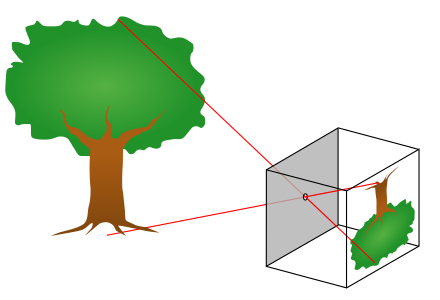
\includegraphics[width=0.48\textwidth]{images/pinhole.png}
			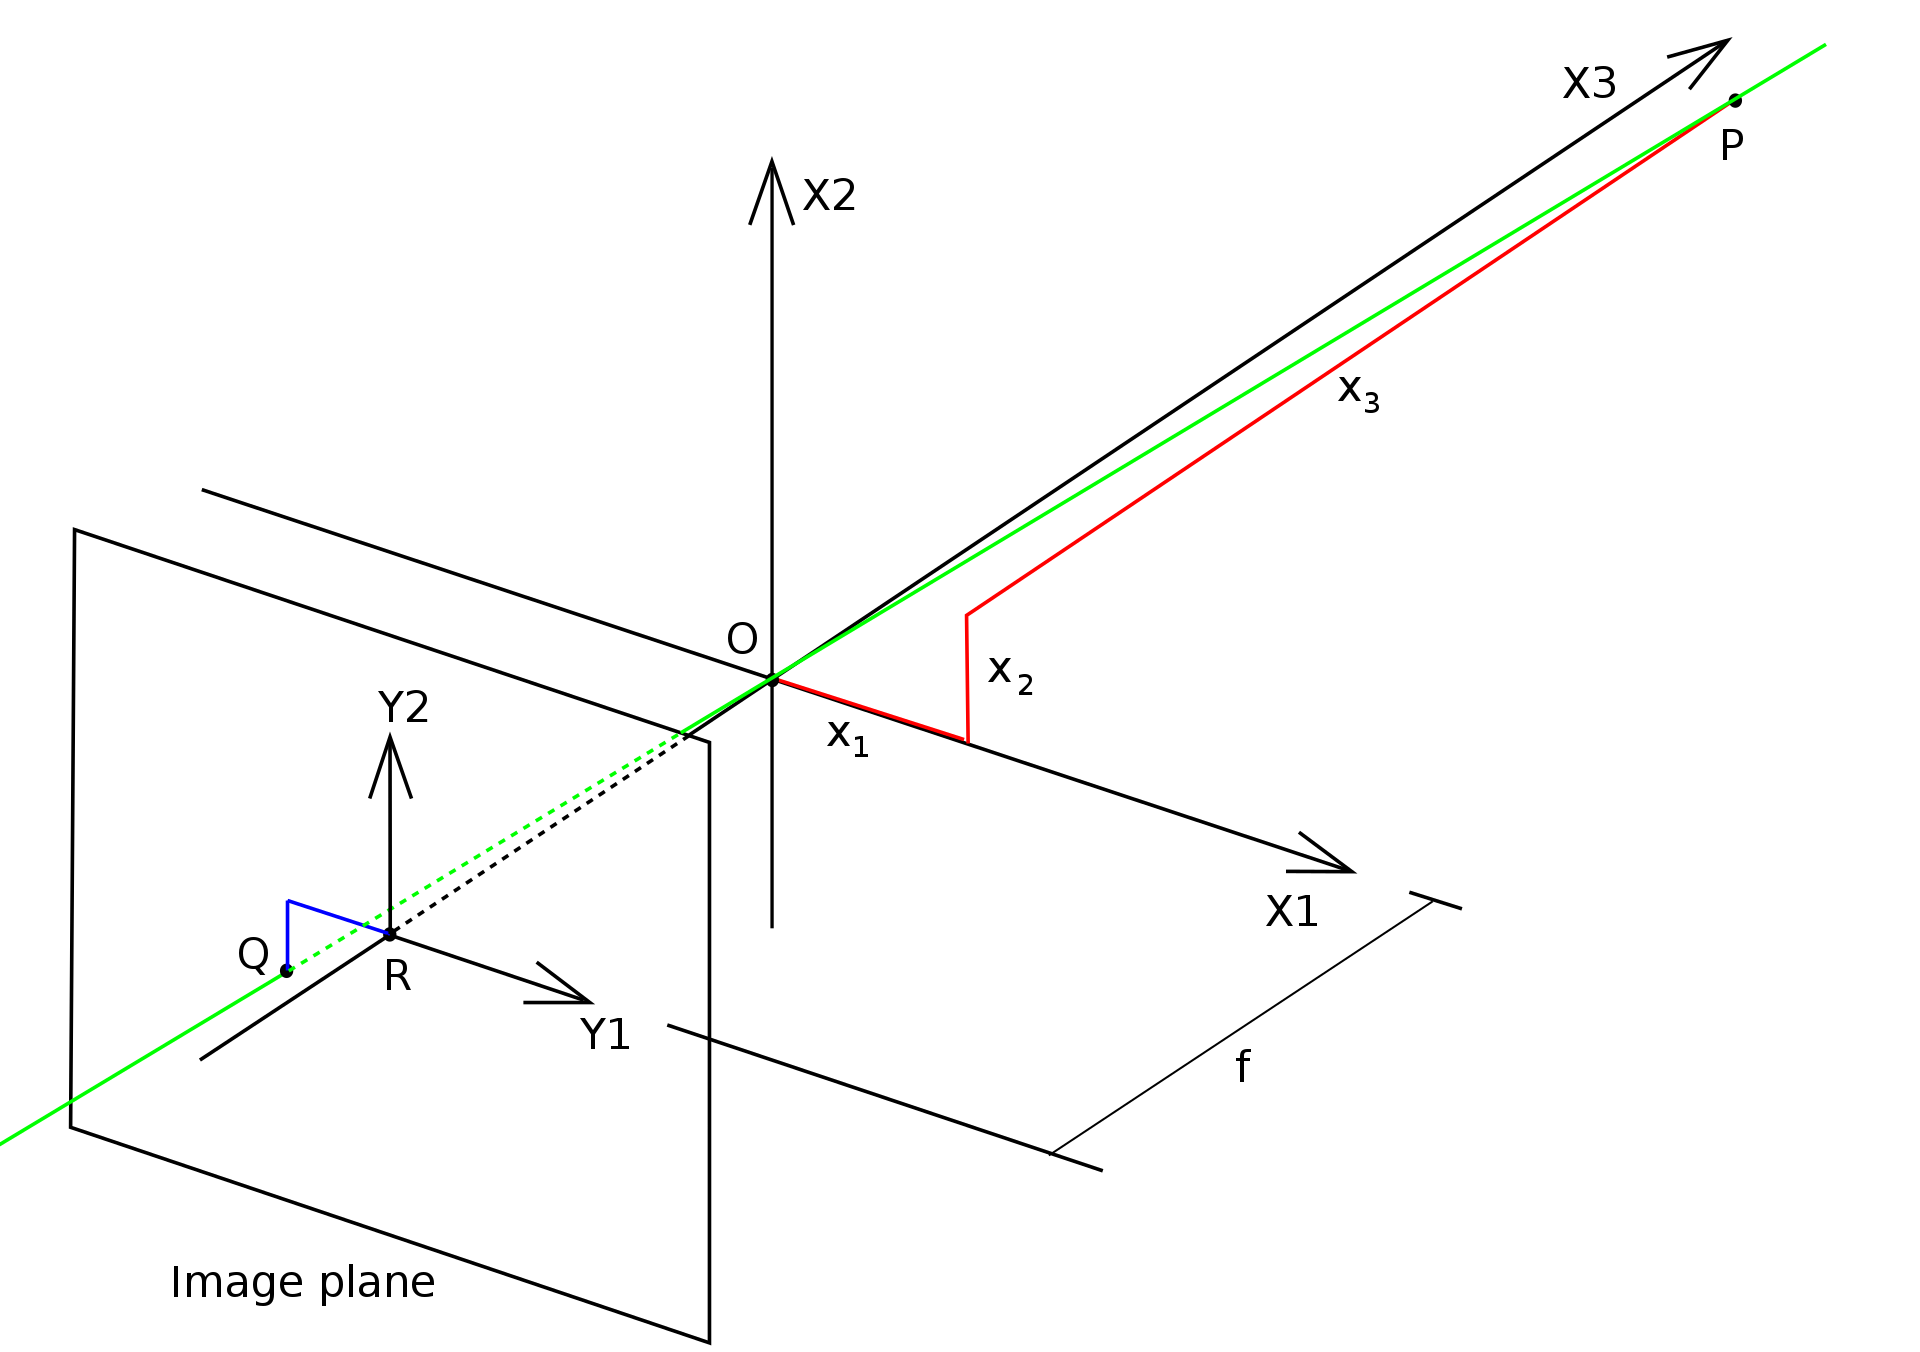
\includegraphics[width=0.48\textwidth]{images/pinhole_coor.png}
		\end{center}
		\caption{成像模型及相机坐标系}
	\end{figure}

	小孔成像又称为透视成像,当我们拍摄平行铁轨时,照片上铁轨不再平行,并且呈近大远小的特点,这就是透视成像的典型特点。\\

	成像过程是一个把空间点投影到像素平面的变换:空间点$P=(x,y,z)$,则根据简单几何知识可知,对应像素坐标为$p = (xf/z, yf/z) = f/z(x,y)$($f$为相机焦距)。\\
	
	注意,$z$不是常数,所以这不是一个线性变换。如果场景点都位于一张平面上,或者场景的深度远远小于场景到相机的距离,可近似认为所有场景点深度都为$z_0$,此时为线性变换,
	$$
		p = \frac{f}{z_0}(x,y)
	$$

	这样的相机称也为\textbf{弱投影相机}或\textbf{仿射相机}。

\subsection{坐标系}
	一般我们要使用到3个坐标系,

	\subsubsection*{世界坐标系}
		世界坐标系用来测量场景的绝对位置,比如可以把原点设置在故宫大殿的中心,这样所有的场景点都会存在一个绝对坐标。\\

		实际上世界坐标只是为了区分不同相机的姿态,没有必要指定一个绝对位置,往往选择第一个相机的坐标系为世界坐标系。

	\subsubsection*{相机坐标系}
		用来刻画场景相对相机光心的姿态,以光心为原点,光轴为$z$轴,以指向场景的方向为正向;\\

		$xy$平面平行于成像平面,上为$y$轴,右为$x$轴,$z-y-x$符合右手法则;\\

		不同的相机对相同场景,会在各自坐标系中刻画出不同的姿态,在世界坐标系中,可以明确相机坐标系之间的转换关系,统一场景的唯一表示。

	\subsubsection*{像素坐标系}
		像素坐标系$uv$就是2D成像平面,单位是像素,平行于相机坐标系的$xy$平面。\\

		$uv$坐标系的原点一般在图像的左下角或左上角,而$xy$平面的原点在光心,也即$uv$平面的中心,在像素坐标系光心存在一个偏移量$c_x,c_y$(单位为像素)。\\

		世界坐标系和相机坐标系的单位是m,而像素坐标系的单位是pixel,在投影的时候需要明确转换因子,即当前相机1m等于多少pixel

\subsection{相机内参矩阵}
	在相机坐标系中,场景成像与相机本身参数有关,这些参数称为\textbf{内参数}。\\

	相机内参数包括下面几种,
	\begin{itemize}
		\item 相机焦距$f$,可以调节成像平面与光心的距离,称为\textbf{物理变焦};焦距大成像大,焦距小成像小
		\item 光心偏移量$c_x,c_y$(单位为像素)
		\item 相机偏斜,因为工艺问题,感光元件构成的像平面不是矩形,存在一个角度$\theta$
		\item $x,y$方向可能存在不同的像素转换因子
	\end{itemize}

	这些参数都考虑进来,得到相机\textbf{内参矩阵},焦距和转换因子已经融合到$\alpha,\beta$参数中,

	\begin{equation}
		K = \begin{bmatrix}
			\alpha \quad& -\alpha\cot\theta        \quad& c_x\\
			0      \quad& \frac{\beta}{\sin\theta} \quad& c_y\\
			0      \quad& 0                        \quad& 1
		\end{bmatrix}
	\end{equation}

	3D点$P$在像素平面的投影可用齐次坐标表示为,

	$$
		P^{\prime} = 
			\left[
				\mathbf{K}\quad \mathbf{0}_{3\times 1}
			\right]
		\begin{bmatrix}
			P\\
			1
		\end{bmatrix} = KP
	$$

	上面得到的$P^{\prime}$是2D平面的齐次坐标,转换为2D坐标还需,
	$$
		p^{\prime} = \begin{bmatrix}
			\frac{K_1P}{K_3P}\\
			\\
			\frac{K_2P}{K_3P}
		\end{bmatrix}
	$$
	$K_1,K_2,K_3$是$K$的行向量。\\

	对任意尺度因子$d$($d\neq 0$),点$dP$的像素坐标为,
	$$
		p_d = \begin{bmatrix}
			\frac{dK_1P}{dK_3P}\\
			\\
			\frac{dK_2P}{dK_3P}
		\end{bmatrix} = p^{\prime}
	$$

	变动$d$,$dP$实际是一条过光心的射线,也就是说射线上所有的点都投影到相同像素上,这也符合直观感受。\\

	也可以认为给$K$乘以因子$d$产生的投影结果不变,这样矩阵称为\textbf{齐次矩阵},只有元素之间的比率有意义。\\

	反之,已知像素平面上一点$p$(齐次坐标),反投影到3D空间会得到一条射线,

	\begin{equation}
		P(d) = dK^{-1}p \label{inverse_proj}
	\end{equation}

\subsection{相机投影矩阵}
	内参矩阵只是刻画在场景相机坐标系下的投影关系,如果场景在世界坐标系下,需要把场景从世界坐标系通过旋转平移变换到相机坐标系,再用内参矩阵进行投影。
	$$
		M = K\left[R\quad T\right]
	$$

	$R,T$为相机坐标系的旋转矩阵和平移向量,$\left[R\quad T\right]$称为相机\textbf{外参矩阵},$M$称为相机的\textbf{投影矩阵}。\\

	投影矩阵是内参矩阵乘以外参矩阵,是一个$3\times 4$的矩阵。\\

	也可以对投影矩阵增广到$4\times 4$的矩阵$\tilde{M}$,

	$$
		\tilde{M} = \begin{bmatrix}
			KR\quad& KT\\
			0\quad& 1
		\end{bmatrix}
	$$

	$\tilde{M}P$投影得到一个$4\times 1$的向量,在代数上这个向量前3维代表像素的齐次坐标,但在几何上没有意义。\\

	增广矩阵主要是能在反投影时简化计算,后面会用到。

\subsection{3D空间的线性变换}

	在MVS任务中要着重研究各个相机成像平面之间的变换关系,下面是3D空间到自身的一些变换(2D空间也类似)。\\

	变换的本质是探究在某些变换群下,那些不变的性质,所以下面每个变换都探讨什么不变。

	\subsubsection{欧式变换}
		对目标进行平移和旋转,保持目标大小、长度、夹角都不变。表示矩阵为,
		$$
			H_E = \begin{bmatrix}
				\mathbf{R}_{3\times 3}\quad& \mathbf{t}_{3\times 1}\\
				0_{1\times 3} \quad& 1_{1\times 1}
			\end{bmatrix}
		$$

		$R$是$3\times 3$的旋转矩阵,$t$是平移向量。\\

		可以验证虚圆点是$H_E$的两个特征向量。这说明欧式变换的本质是虚圆点不变,大小、长度、夹角都是因为虚圆点不变而成立。\\

		\textit{2D欧式变换有3个自由度,3D的有6个自由度}

	\subsubsection{相似变换}
		均匀缩放的欧式变换,目标大小、长度发生变化,但夹角不变,
		$$
			H_S = \begin{bmatrix}
				s\mathbf{R}_{3\times 3}\quad& \mathbf{t}_{3\times 1}\\
				0_{1\times 3} \quad& 1_{1\times 1}
			\end{bmatrix}
		$$

		$s$是缩放尺度,3个方向上相同。可以验证,虚圆点也是相似变换的特征向量。\\

		\textit{2D相似变换有4个自由度,3D的有7个自由度}
	
	\subsubsection{仿射变换}
		非均匀缩放的欧式变换,夹角不能保持,但能保持平行线变换后仍为平行,无穷远平面不变。
		$$
			H_A = \begin{bmatrix}
				\mathbf{A}_{3\times 3}\quad& \mathbf{t}_{3\times 1}\\
				0_{1\times 3} \quad& 1_{1\times 1}
			\end{bmatrix}
		$$

		$A$是一个可逆矩阵。\\

		标准无穷远平面$\pi_{\infty} = (0,0,0,1)^T$,根据点面对偶原理,平面变换为,
		\begin{align*}
			\pi_{\infty}^{\prime} = H_A^{-T}\pi_{\infty} 
			&=
			\begin{bmatrix}
				\mathbf{A}_{3\times 3}\quad& \mathbf{t}_{3\times 1}\\
				0_{1\times 3} \quad& 1_{1\times 1}
			\end{bmatrix}^{-T}
			\begin{bmatrix}
				\mathbf{0}_{3\times 1}\\
				1
			\end{bmatrix}\\
			&=
			\begin{bmatrix}
				\mathbf{A}^{-T}\quad& \mathbf{0}\\
				-\mathbf{t}^TA^{-T} \quad& 1
			\end{bmatrix}
			\begin{bmatrix}
				\mathbf{0}\\
				1
			\end{bmatrix}\\
			&= (0,0,0,1)^T\\
			&=\pi_{\infty} 
		\end{align*}

		很容易验证,无穷远直线(2D)/无穷远面(3D)是仿射映射的特征向量。仿射变换可分解为(以2D为例),
		$$
			\mathbf{A} = \mathbf{R}(\theta)\mathbf{R}(-\phi)
			\begin{pmatrix}
				s_x \quad &0\\
				0 \quad & s_y
			\end{pmatrix}
			\mathbf{R}(\phi)
		$$

		$s_x,s_y$为在$x,y$方向的放缩因子,$\theta,\phi$为旋转角度,如此可以看出仿射变换的确是非均匀缩放的欧式变换。\\

		\textit{2D仿射变换有6个自由度,3D的有12个自由度}
	
	\subsubsection{射影变换}

		\textbf{射影变换} 又称为 \textbf{单应变换},这两个名字会混着用。\\

		具有更一般的形式,平行性和无穷远平面也保持不了,但能保持线性性,即直线仍映射为直线。
		$$
			H_P = \begin{bmatrix}
				\mathbf{A}_{3\times 3}\quad& \mathbf{t}_{3\times 1}\\
				\mathbf{v}_{1\times 3} \quad& 1_{1\times 1}
			\end{bmatrix}
		$$

		以2D为例,对直行$x^Tl = 0$,变换后的点$x^\prime = H_Px$,变换后的$l^\prime = H_P^{-T}l$,

		$$
			x^\prime l^\prime = \left(H_Px\right)^TH_P^{-T}l = x^T H_P^TH_P^{-T}l = 0
		$$

		2D空间中的确直线变为直线。3D空间的直线表示比较复杂,需用两个平面交线表示:$x^T\pi_A =0,  x^T\pi_B =0$,
		\begin{align*}		
			x^\prime \pi_A^{\prime} &= (H_Px)^T(H_P^{-T}\pi_A) = x^TH_P^TH_P^{-T}\pi_A = 0\\
			x^\prime \pi_B^{\prime} &= (H_Px)^T(H_P^{-T}\pi_B) = x^TH_P^TH_P^{-T}\pi_B = 0
		\end{align*}

		所以3D空间的线性性也得到保证。如下情况会存在平面间的射影变换,

		\begin{itemize}
			\item 场景如果是平面,则场景平面与像平面间的变换
			\item 场景是平面,则不同相机的成像平面之间的变换
			\item 同一相机,只有旋转没有平移拍摄到的像平面之间的变换;这种拍摄方式常用来做广角图拼接
			\item 同一光心透视两张平面之间形成的变换
		\end{itemize}

		如果场景不是平面,则不同相机像平面之间一般不是射影变换,会用更一般的极几何约束这种对应关系。\\

		射影变换可以进行层次化分解,$\mathbf{H} = \mathbf{H_S}\mathbf{H_A}\mathbf{H_P}$,
		$$
			\begin{pmatrix}
				\mathbf{A}_{3\times 3}\quad& \mathbf{t}_{3\times 1}\\
				\mathbf{v}_{1\times 3} \quad& 1_{1\times 1}
			\end{pmatrix}
			=
			\begin{pmatrix}
				s\mathbf{R}_{3\times 3}\quad & \mathbf{t}_{3\times 1}\\
				\mathbf{0}_{1\times 3}\quad & 1_{1\times 1}
			\end{pmatrix}
			\begin{pmatrix}
				\mathbf{K}_{3\times 3}\quad & \mathbf{0}_{3\times 1}\\
				\mathbf{0}_{1\times 3}\quad & 1_{1\times 1}
			\end{pmatrix}
			\begin{pmatrix}
				\mathbf{I}_{3\times 3}\quad & \mathbf{0}_{3\times 1}\\
				\mathbf{v}_{1\times 3}\quad & 1_{1\times 1}
			\end{pmatrix}
		$$
		\textit{2D透视变换有7个自由度,3D的有15个自由度}
	\subsubsection{仿射恢复}

		仿射变换使得无穷远点保持不变,而射影变换则使得无穷远点变为有限点,如下图\footnote{\url{https://www.graphicsmill.com/docs/gm/affine-and-projective-transformations.htm}},

		\begin{figure}[H]
			% \begin{center}
			\begin{minipage}[t]{0.52\linewidth}
				\centering
				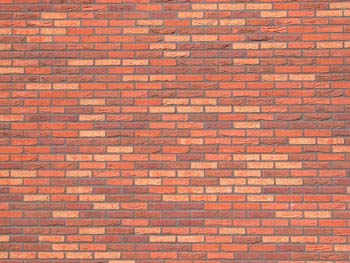
\includegraphics[width=0.8\textwidth]{images/origin_.jpeg}
				\caption{墙面原图}
			\end{minipage}
			\begin{minipage}[t]{0.78\linewidth}
				\centering
				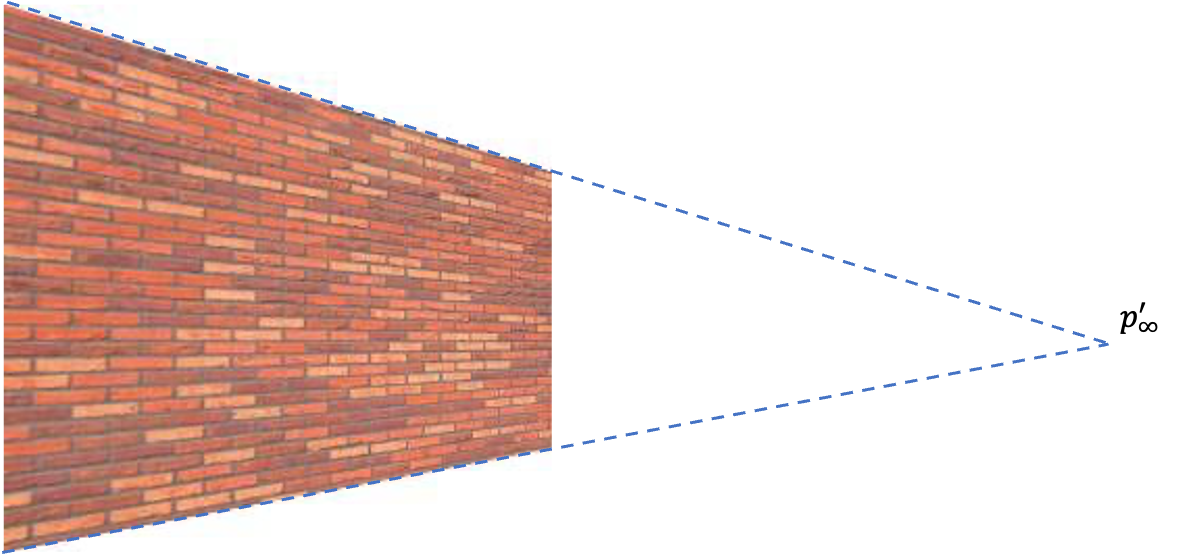
\includegraphics[width=0.8\textwidth]{images/projective_.png}
				\caption{射影变换,无穷远点被映射为有限点}
			\end{minipage}			
		\end{figure}

		可以把无穷远点的像$p^{\prime}_{\infty}$映射回标准位置$(0,0,1)$,来恢复图像的仿射性质,具体来说,

		$$
			\mathbf{H}\mathbf{H_P}^{-1} = \mathbf{H_S}\mathbf{H_A}
		$$

		只要在图像上测量$p^{\prime}_{\infty}$的像素坐标,便可纠正图像的射影失真,恢复仿射性质,

		\begin{figure}[H]
			\begin{minipage}[t]{0.52\linewidth}
				\centering
				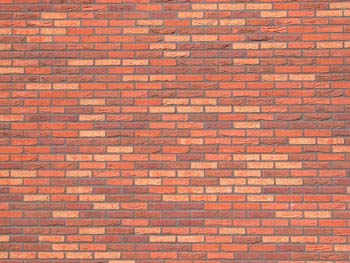
\includegraphics[width=0.8\textwidth]{images/origin_.jpeg}
				\caption{墙面原图}
			\end{minipage}		
			\begin{minipage}[t]{0.5\linewidth}
				\centering
				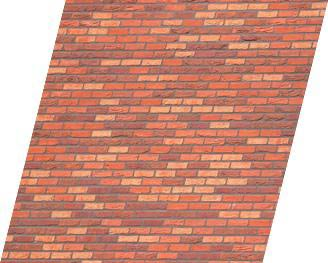
\includegraphics[width=0.8\textwidth]{images/affine_.jpeg}
				\caption{仿射恢复,通过无穷远点消除射影失真}
			\end{minipage}			
		\end{figure}
		
		如果观察到更多的条件,可以继续消除仿射失真,恢复欧式性质。这就是变换的层次分解带来的好处。

\subsection{反称矩阵}
 	向量$\mathbf{u},\mathbf{v}$的叉乘,
 	\begin{align*}
 		\mathbf{u}\times \mathbf{v} &= 
 		\begin{vmatrix}
 			\mathbf{i}\quad & \mathbf{j}\quad & \mathbf{k}\\
 			u_1\quad& u_2\quad& u_3\\
 			v_1\quad& v_2\quad& v_3
 		\end{vmatrix}\\
 		&= (u_2v_3 -u_3v_2)\mathbf{i} + (u_3v_1 - u_1v_3)\mathbf{j} +(u_1v_2 - u_2v_1)\mathbf{k}\\
 		&=\begin{bmatrix}
 			0 \quad& -u_3\quad & u_2\\
 			u_3\quad & 0\quad& -u_1\\
 			-u_2\quad& u_1\quad& 0
 		\end{bmatrix}
 		\begin{bmatrix}
 			v_1\\
 			v_2\\
 			v_3
 		\end{bmatrix}
 		\\
 		&= [\mathbf{u}]_{\times} \cdot \mathbf{v}
 	\end{align*}

 	$[\mathbf{u}]_{\times}$为由$\mathbf{u}$张成的\textbf{反称矩阵},
 	$$
 		[\mathbf{u}]_{\times} = 
 		\begin{bmatrix}
 			0 \quad& -u_3\quad & u_2\\
 			u_3\quad & 0\quad& -u_1\\
 			-u_2\quad& u_1\quad& 0
 		\end{bmatrix}
 	$$

	这个矩阵存在如下性质,

	\begin{itemize}
		\item 对任意向量$p$,$p^T [\mathbf{u}]_{\times} p = 0$
		\item 矩阵秩为2,特征值为和纯虚数;所以基础矩阵秩为2
		\item 二次幂可展开为,
			$$
				[\mathbf{u}]_{\times}^2 = \mathbf{u}\mathbf{u}^T - \Vert\mathbf{u}\Vert^2 \mathbf{I_3}
			$$
		\item 三次幂等价于自身,
			$$
				[\mathbf{u}]_{\times}^3 = -\Vert\mathbf{u}\Vert^2[\mathbf{u}]_{\times}
			$$
		\item 对任意向量$\mathbf{t}$和非奇异矩阵$\mathbf{M}$,
			\begin{equation}
				[\mathbf{t}]_{\times}\mathbf{M} = \mathbf{M}^{-T}\left[\mathbf{M}^{-1}t\right]_{\times} \label {inver_m_p}
			\end{equation}
	\end{itemize}

\section{对极约束}
	如前所述,对一般场景而言,两个成像平面构不成射影变换,它们服从更一般的\textbf{极几何}约束,可用一个矩阵$F$表示这种约束关系,矩阵$F$称为\textbf{基础矩阵},
	\begin{figure}[H]
		\begin{center}
			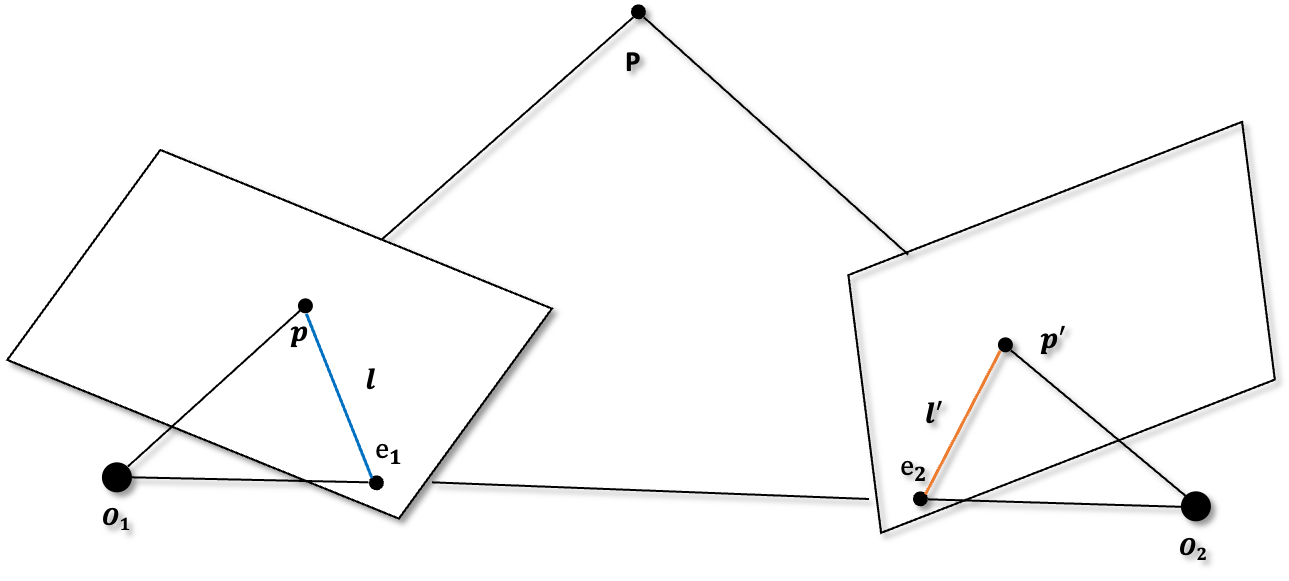
\includegraphics[width=0.8\textwidth]{../images/base_matrix.png}
		\end{center}
		\caption{两图像之间的极几何约束,$O_1,O_2$为相机\textbf{光心},$O_1O_2$为\textbf{基线},$p,p^{\prime}$为$P$在两个像素平面的像,$e,e^\prime$为\textbf{极点},$l,l^{\prime}$为\textbf{极线}}
	\end{figure}
	\begin{itemize}
		\item 世界坐标系选为第一个相机坐标系
		\item $K,K^{\prime}$是两个相机的内参矩阵
		\item $R,T$是第二个相机相对第一个相机的旋转和平移
		\item $[T]_{\times}$是$T$张成的反称矩阵,秩为$2$
		\item $e,e^\prime$为极点,$e^\prime$是$e$及原点$(0,0,0)$的投影,存在
			$$
				e^\prime = K^\prime[R \quad T]\begin{bmatrix}
					\mathbf{0}\\
					1
				\end{bmatrix} = K^\prime T
			$$	
	\end{itemize}

	所有极线都过极点,所以,
	$$
		{p^\prime}^T l^\prime = 0, \quad {e^\prime}^T l^\prime = 0
	$$
	\subsection*{基础矩阵}
		$p,p^\prime$是同一个空间点$P$在两个像素平面的投影,将$p$反投影到$P$,再投影到第二个像素平面可得到$p^\prime$,根据(\ref{inverse_proj}),

		\begin{align}
			p^{\prime}_d &= K^{\prime}[R\quad T]
			\begin{bmatrix}
				dK^{-1}p\\
				1
			\end{bmatrix}\nonumber\\
			&= K^{\prime}\left(dRK^{-1}p + T\right)\nonumber\\
			&= dK^{\prime}RK^{-1}p + K^{\prime}T\label{f_inverse}\\
			&= dK^{\prime}RK^{-1}p + e^\prime\label{f_inverse_e}
		\end{align}

		尺度因子$d$在齐次坐标下并无影响,只是提醒反投影后存在一个尺度。\\

		由此可见,一般情况下$p,p^\prime$之间并非射影变换。\\

		(\ref{f_inverse_e})式两边叉乘$e^\prime$,

		$$
			p^{\prime}_d\times e^\prime = dK^{\prime}RK^{-1}p \times e^\prime
		$$

		转置一下,
		$$
			e^\prime \times p^{\prime}_d = e^\prime \times dK^{\prime}RK^{-1}p = d[e^\prime]_{\times}K^{\prime}RK^{-1}p
		$$

		两边与$p^\prime_d$作内积,
		$$
			p^\prime_d [e^\prime]_{\times}K^{\prime}RK^{-1}p = 0
		$$

		称,
		\begin{equation*}
			\mathbf{F} = [e^\prime]_{\times}K^{\prime}RK^{-1}
		\end{equation*}

		为\textbf{基础矩阵},任意点对$p^\prime,p$都满足约束,

		\begin{equation}
			{p^{\prime}}^T \mathbf{F} p = 0 \label{f_constrain}
		\end{equation}

		根据(\ref{inver_m_p}),可得到$F$的另一表达式,

		$$
			\mathbf{F} = [e^\prime]_{\times}K^{\prime}RK^{-1} = {K^{\prime}}^{-T}[T]_{\times}RK^{-1}
		$$

		下面两个表达式都是$F$的常用形式,
		\begin{align}
			\mathbf{F} &= [e^\prime]_{\times}K^{\prime}RK^{-1} \label{f_1}\\
			\mathbf{F} &= {K^{\prime}}^{-T}[T]_{\times}RK^{-1} \label{f_1}
		\end{align}

		$[T]_{\times},[e^\prime]_{\times}$的秩为2,所以$F$的秩也为2。\\

	\subsection*{基础矩阵求解}
		基础矩阵$F$有$7$个自由度,这个点可以从两方面看出,
		\begin{itemize}
			\item \textbf{直接法},内参矩阵$K,K^\prime$已知,平移向量$T$有3个自由度,旋转矩阵$R$有4个自由度(绕某轴转某角),所以总共7个自由度
			\item \textbf{间接法},$F$是$3\times 3$矩阵,总共9个变量,一消去个不重要的尺度因子,所以总共8个变量;考虑秩为2,再消去一个变量,所以总共7个自由度
		\end{itemize}

		令$p=[x_1,x_2,1]^T,p^\prime = [x_1^\prime,x_2^\prime,1]$,

		\begin{equation}
			{p^{\prime}}^T \mathbf{F} p = 0
		\end{equation}

		可整理成,
		$$
			a\cdot f = 0
		$$

		\begin{align*}
			a &= [x_1^\prime x_2^\prime,x_1^\prime x_2,x_1^\prime, x_1x_2^\prime,x_1x_2,x_1,x_2^\prime,x_2,1]\\
			f &= [f_{11},f_{12},f_{13},f_{21},f_{22},f_{23},f_{31},f_{32},f_{33}]^T
		\end{align*}

		$a$是一对观测点$(p,p^\prime)$,$n$对点则会构成一个矩阵$D_{n \times 9}$,可构成线性方程,

		\begin{equation}\label{f_matrix_eq}
			Df = 0
		\end{equation}

		$D$称为\textbf{观测矩阵},一般通过特征匹配来确定,在SfM中属于已知量。\\

	\subsubsection*{七点法}

		一对点构造一个方程,所以7对点即可精准求解除$F$,称为\textbf{七点法}。\\

		$f$的通解为
		$$
			f = \lambda f_1 + \mu f_2
		$$

		$F$是一个齐次向量,尺度不重要,可归一化为,
		
		$$
			f = \lambda f_1 + (1-\lambda) f_2
		$$

		以及,
		$$
			F = \lambda F_1 + \mu F_2
		$$

		其中$f_1,f_2$是矩阵$D$零空间的两个基向量($D$有7个自由度,所以零空间维度为2),$F_1,F_2$为$f_1,f_2$对应的非0矩阵。\\

		因为$F$的秩为2,因此,$\det(F) = 0$,所以

		$$
			\det(\lambda F_1 + (1-\lambda) F_2) = 0
		$$

		注意$f_1,f_2,F_1,F_2$都是确定的,上面行列式展开便可求出$\lambda$,从而求出$F$。\\

		但上式展开是一个关于$\lambda$的三次函数,会得到三个根,需要排除复根和相机后面的点,从而得出正确的解。

	\subsubsection*{八点法}	
		\textbf{七点法}虽能准确求解基础矩阵,但运算过程是麻烦的,并且在实际中数据会存在噪音,只用7个点得到的解也会存在噪音。\\

		所以通常考虑多于7对点来确定基础矩阵,比如\textbf{八点法}。\\

		此时,方程(\ref{f_matrix_eq})是超定的,可转变为最小化问题,
		$$
			\min \Vert Df\Vert^2 ,\quad s.t. \quad \Vert f\Vert = 1
		$$

		这个问题变得很简单,$f$就是$D$作奇异值分解后,右奇异矩阵的最后一列。

	\subsection*{点线对应}

		$p^{\prime}$在极线$l^{\prime}$上,而$p^\prime \mathbf{F} p=0$,可知,

	\begin{align*}
		l^{\prime} = Fp,\quad 
		l = F^Tp^\prime
	\end{align*}

	基础矩阵描述了点之间的约束关系,每个点对应一条极线。\\

	极点$e^\prime$在所有极线$l^\prime$上,故,
	$$
		{e^\prime}^T l^\prime = 0 \Rightarrow {e^\prime}^TFp=0 
	$$

	因为$p$的任意性,可知

	$$
		{e^\prime}^T F = 0, \quad Fe = 0
	$$

	沿着极线$l^\prime$搜索$p$的像,会大幅缩小搜索范围。

	\subsection*{工程实现}
		在实际计算时,通过投影矩阵的增广的投影矩阵表示更为方便,
		\begin{equation}
			N_d= M^{\prime}M^{-1} = \begin{bmatrix}
				dK^\prime R K^{-1} \quad& K^\prime T\\
				0\quad& 1\quad
			\end{bmatrix}\label{extend_f}		
		\end{equation}

		从$N_d$中截取出左上角$3\times 3$的矩阵便是旋转矩阵,右上角$3\times 1$的向量是平移向量,这在各种工具中非常容易实现。

\section{外参恢复}\label{section_recovery_outer_p}
	基础矩阵$F$包含了相机的内外参数,如果相机内参已知,能否从$F$中分离出外参?\\

	$$
		\mathbf{F} = {K^{\prime}}^{-T}[T]_{\times}RK^{-1} \Rightarrow {K^{\prime}}^{T}\mathbf{F} K = [T]_{\times}R = \mathbf{E}
	$$

	其中,
	$$
		\mathbf{E} = [T]_{\times}R
	$$

	称为\textbf{本质矩阵}。现在问题简化为如何从$E$中分离出外参$R,T$。\\

	根据(\ref{inverse_decompose}),$[T]_{\times}$可分解为,

	\begin{align*}
		[T]_{\times} &= U diag(1,1,0)WU^T\\
		[T]_{\times} &= U diag(1,1,0)W^TU^T
	\end{align*}

	这两种分解仅差一个尺度或者符号。$E$可表示为,

	\begin{align*}
		\mathbf{E} = U diag(1,1,0)\left(WU^TR\right)\quad 
		\text{or} \quad 
		U diag(1,1,0)\left(W^TU^TR\right)
	\end{align*}

	注意$E$是秩为2的反称矩阵,奇异值分解形式为,

	$$
		\mathbf{E} = U diag(1,1,0) V^T
	$$

	在$\mathbf{E} $确定的情况下,$U,V$是已知量,对比可知,
	\begin{align*}
		V^T = WU^TR \quad \text{or}\quad W^TU^TR
	\end{align*}

	得到$R$的两种表达式,
	\begin{align*}
		R = UW^TV^T\quad \text{or}\quad UWV^T
	\end{align*}

	$R$是旋转矩阵,所以行列式值为正,修正一下符号,

	$$
		R \leftarrow (\mathop{det} R)R
	$$

	而,
	$$
		[T]_{\times} = R^T\mathbf{E}
	$$

	这样得到$T$的反称矩阵,可以组合出$T$向量;$R$有两个值,$T$也对应有两个值。\\


	这两组解几何表示,一组场景都在相机前面;一组场景在相机后面,通过重建出的点过滤掉在后面的解即可。

\section{单应变换}

	如果拍摄场景是一张平面,法向量为$\mathbf{n}$,到原点距离为$d$,则平面方程为,
	$$
		\mathbf{n}^T P = d
	$$

	$\mathbf{n}_d = \mathbf{n}/d$,场景平面可表示为,
	
	$$
		\mathbf{n}_d^T P = 1
	$$

	像素点$p$反投影为$dK^{-1}p$,

	\begin{align*}
		p^{\prime}(d) &= K^{\prime}\left(dRK^{-1}p + T\right)\\
		&= K^{\prime}\left(dRK^{-1}p + T\mathbf{n}_d^T P\right)\\
		&= K^{\prime}\left(dRK^{-1}p + T\mathbf{n}_d^TdK^{-1}p\right)\\
		&= dK^{\prime}\left(R + T\mathbf{n}_d^T\right)K^{-1}p\\
		&= Hp
	\end{align*}

	这里的关键是第二步,代入场景平面方程,把$p$给分离了出来,$p^\prime,p$之间构成射影变换。\\

	$K^\prime$是齐次矩阵,与$dK^\prime$等价。

	\begin{equation}
		H= K^{\prime}\left(R + T\mathbf{n}_d^T\right)K^{-1} \label{homograph_matrix}
	\end{equation}

	称为\textbf{单应矩阵},因此射影变换也称为\textbf{单应变换}。\\

	$p,p^{\prime}$依然服从基础矩阵的约束,(\ref{extend_f})式的增广表示也包含了单应变换这一特殊情况。\\

	基础矩阵只是描述点与极线的对应关系,而单应矩阵描述点之间一一对应关系,这也是“\textbf{单应}”的意义。

	\subsection*{论文中的公式}

	在MVSNet中,只知道两个相机在世界坐标系的旋转和平移$R_1,t_1,R_2, t_2$,相对旋转$R$和平移$t$为,

	$$
		R = R_2R_1^{-1},\quad 
		t = t_2 - R_2R_1^{-1}t_1
	$$

	(\ref{homograph_matrix})用世界坐标系可表示为,

	\begin{align}
		H &= K_2 \left(R_2R_1^{-1} +\left(t_2 - R_2R_1^{-1}t_1\right) \mathbf{n}_d^T\right) K_1^{-1} \label{new_homograph_matrix}
	\end{align}	

	原论文中的公式是错误的,这是正确版本。\\

	增广表示蕴含了单应变换,这个复杂的式子在编程中并不会被使用到。

\bibliography{math}
\end{document}